\input{style/settings}
\input{style/short_commands}
\pagestyle{fancy}
\fancyhf{}
\fancyhead[R]{página\;\thepage/\pageref{LastPage}}
\fancyhead[L]{Osvaldo Uriel Calderón Dorantes}
\fancyfoot[L]{Seguridad Radiológica}
\fancyfoot[R]{Facultad de Ciencias, UNAM 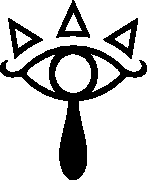
\includegraphics[scale=0.13]{style/Sheikah.pdf}}
\fancypagestyle{plain}{
  \fancyfoot[C]{}
}
\makeatletter
\def\@seccntformat#1{%
  \expandafter\ifx\csname c@#1\endcsname\c@section\else
  \csname the#1\endcsname\quad
  \fi}
\makeatother
%%%%%%%%%%%%%%%%%%%%%%%%%%%%%%%%%%%%%%%%%%%%%%%%%%%%%%%
%%%%%%%%%%%%%%%%%%%%%%%%%%%%%%%%%%%%%%%%%%%%%%%%%%%%%%%%%%%
\begin{document}
\begin{flushleft}
Osvaldo Uriel Calderón Dorantes, \hfill Seguridad Radiológica\\
316005171 \hfill osvaldo13576@ciencias.unam  \\
Facultad de Ciencias\\
\underline{Universidad Nacional Autónoma de México}
\end{flushleft}

\begin{flushright}\vspace{-5mm}

\includegraphics[height=1.5cm]{style/logo.pdf}
\end{flushright}
 
\begin{center}\vspace{-1cm}
\textbf{ \large \customfont{Tarea 2}}\\
%\today
25 de febrero 2022
\end{center}
%\medskip\hrule\medskip
%%%%%%%%%%%%%%%%%%%%%%%%%%%%%%%%%%%%%%%%%%%%%%%%
%{\small \textbf{Nota: A las unidades las pondré dentro de corchetes \ec{\cor{\tx{\customfont{UNIDAD}}}} para no confundir entre variables y realizar el análisis dimensional fácilmente.}}
\medskip\hrule\bigskip

\newlength{\strutheight}
\settoheight{\strutheight}{\strut}
\begin{enumerate}[1.]
  \item ¿Qué es un puente de hidrógeno?
  
  \begin{figure}[!ht]
    \begin{center}
      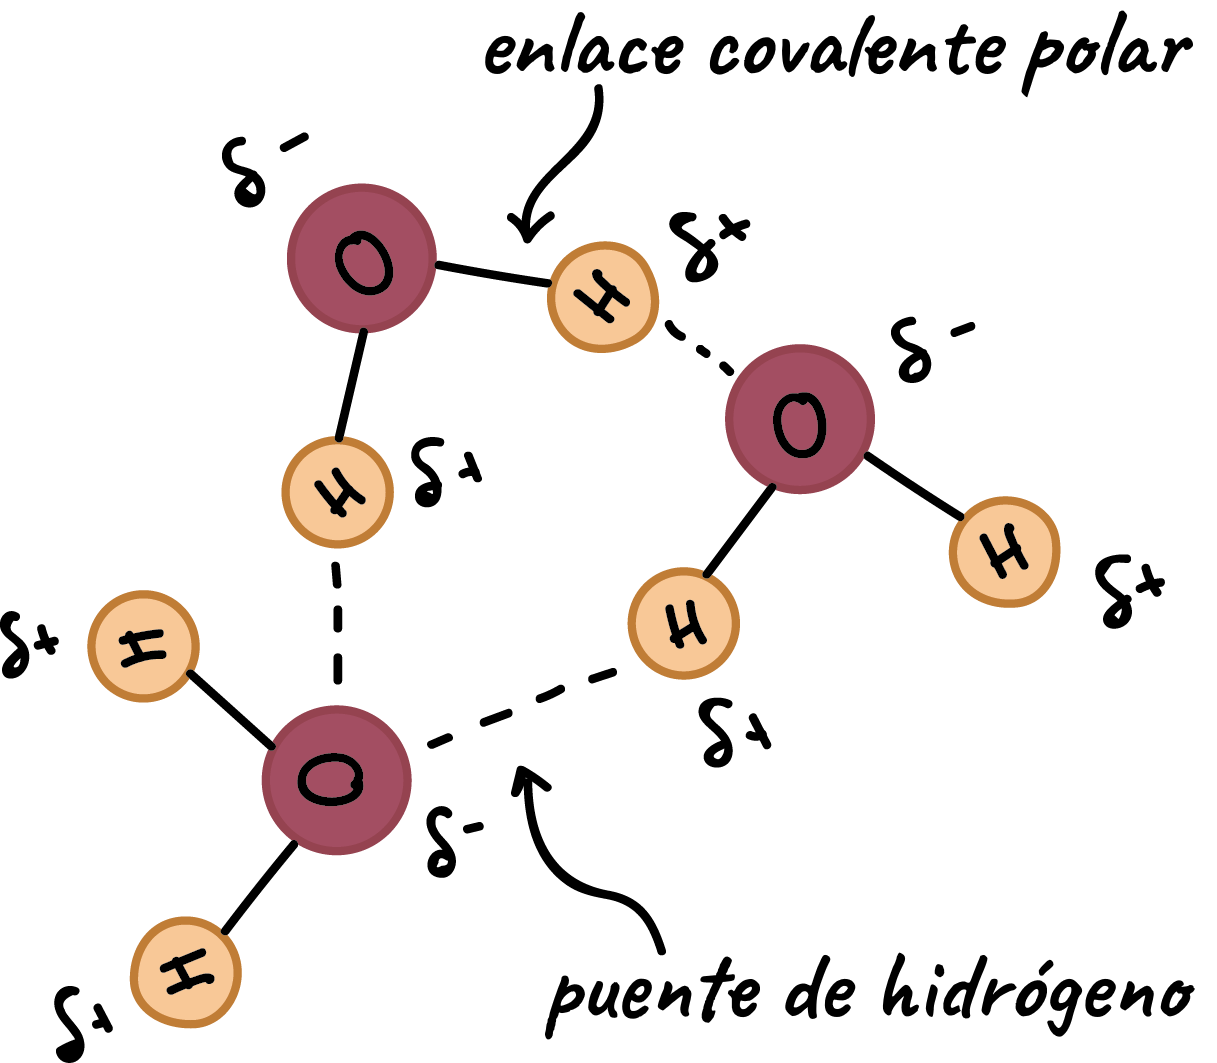
\includegraphics[width=0.24\textwidth]{figuras/ph.png}
    \end{center}
    \caption{Ilustración de un puente de hidrógeno, figura recuperada de \url{https://es.khanacademy.org/science/ap-biology/chemistry-of-life/structure-of-water-and-hydrogen-bonding/a/hydrogen-bonding-in-water}.}
    \label{f:1}
  \end{figure}

  El puente de hidrógeno un tipo de enlace químico intermolecular, donde hay un tipo de unión entre moléculas. Este enlace se trata de una atracción electrostática entre átomos de hidrógeno parcialmente positivos \ec{\delta^+} con átomos átomos parcialmente negativos \ec{\delta^-}, los cuales pueden ser con átomos de flúor, oxígeno o nitrógeno. Como ejemplo, consideramos al agua en la figura \ref{f:1}, el agua \ec{H_2O} es una molécula polar ya que tiene una distribución de carga desigual, en el hidrógeno estará la carga parcial positiva, mientras que en el oxígeno estará la carga parcial negativa.


  \item Define el enlace tipo Van der Waals.
  
Este enlace también es de tipo intermolecular, éstos son débiles a diferencia de los puentes de hidrógeno. En las uniones de este tipo, las moléculas pueden ser atraídas a distancias moderadas mientras que se repelen a cortas distancias, de manera colectiva este conjunto de fuerzas se le conoce como fuerza de Van der Waals. Este tipo de enlace resulta de la suma entre fuerzas de atracción y repulsión entre átomos y moléculas, entonces el enlace se mantendrá mientras que la fuerza de atracción sea mayor que la fuerza de repulsión. 



  \item Configuración electrónica del átomo elegido:
  \begin{figure}[!ht]
    \begin{center}
      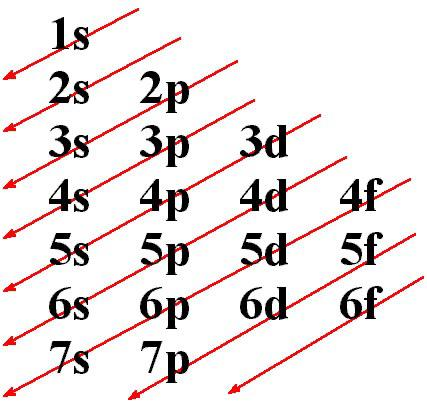
\includegraphics[width=0.24\textwidth]{figuras/fig_conf_elec.png}
    \end{center}
    \caption{}
    \label{f:3}
  \end{figure}

Elemento asignado: \ec{35+N}, \ec{N=4} mi número de lista, átomo asignado 39, Itrio. Según la figura \ref{f:3} se van llenando los electrones según la regla diagonal hasta obtener el número igual de electrones que de protones, suponiendo un átomo eléctricamente neutro. 

\ecc{1s^2 \;2s^2 \;2p^6 3s^2 \;3p^6 \;3d^{10} \;4s^2 \;4p^6 \;4d^1 \;5s^2}


\end{enumerate}


%\begin{multicols}{2}
%\small{\bibliographystyle{apalike}
%\bibliography{bib}}
%\end{multicols}



%\ftikz{1.5}{figuras/fig.tikz}{}{fig:x}

\end{document}



}